% Aufrufen mit: TEXINPUTS=minted/source: xelatex -shell-escape blatt-python.tex
\documentclass{blatt}
\let\raggedsection\centering

\usepackage{fontspec,xunicode}
\usepackage[osf]{mathpazo}
\usepackage[T1]{fontenc} %EU1?
%\defaultfontfeatures{Mapping=tex-text}
%\setmainfont{Linux Libertine O}

\usepackage{minted}
\setminted{linenos}

\newcommand{\XXX}[1]{\textbf{XXX:} #1}

\newsavebox{\foobox}

\begin{document}

\maketitle{Python, eine moderne Programmiersprache}

\tableofcontents

\section{Was ist Python?}

Python ist eine moderne Programmiersprache, die sich bei vielen Entwicklerinnen
und Entwicklern großer Beliebtheit erfreut. Sie wurde Anfang der 90er Jahre von
Guido van Rossum, einem niederländischen Programmierer, entworfen und wird seitdem
von einer großem Team Freiwilliger als freies Open-Source-Projekt gepflegt.

Python ist eine so genannte höhere Programmiersprache, die die Zeit der
Programmiererin oder des Programmierers über die Zeit des Computers stellt.
Gelegentlich ist Python-Code also etwas langsamer als zum Beispiel mühsam
handoptimierter C-Code -- dafür lässt es sich in Python viel schneller und
angenehmer entwickeln.

Zu den Anwendungsbereichen von Python gehören unter anderen die Web-, System-
und Spiele-Entwicklung. Außerdem wird Python für wissenschaftliche Zwecke
eingesetzt -- das ist der Aspekt, den wir beleuchten werden.


\section{Installation von Python}

Damit ein Computer Python-Programme ausführen kann, muss man zunächst einen
\emph{Python-Interpreter} installieren. Das ist die erste Aufgabe an dich!

\paragraph{Unter Ubuntu Linux und anderen Debian-Derivaten.}
Öffne eine Konsole und setz den Befehl \texttt{sudo apt-get install
python-numpy python-scipy python-matplotlib} ab. Das war's schon.

\paragraph{Unter Mac OS X und Windows.} Lade auf
\url{http://continuum.io/downloads} das Komplettpaket Anaconda herunter und
klicke dich durch die Installation. Wähle die Python-Version~2.7 und unter
Windows die 32-Bit-Version (auch, wenn dein Computer ein 64-Bit-Prozessor haben
sollte).

\paragraph{Übers Internet.} Wenn du Schwierigkeiten bei der Installation hast,
schreib uns bitte an. In der Zwischenzeit kannst du aber auch übers Internet
unseren Python-Server verwenden; dann musst du auf deinem eigenen Computer
nichts installieren. Gehe dazu in einem Browser deine Wahl auf
\url{http://speicherleck:????/}. Das Passwort lautet \texttt{XXX}. Bitte
beachte: Das ist unser privater Server, und wir haben ihn nicht besonders
gesichert. Du könntest also prinzipiell in unseren Dateien schnüffeln oder sie
löschen. Bitte mach das nicht! \texttt{:-)}


\section{Erste Schritte}

Mit diesen Notizen möchten wir dir die Grundlagen der Python-Programmierung
beibringen. Wenn du bisher noch keine Programmiersprache beherrschst, wirst du
feststellen, dass das Erlernen gar nicht so einfach ist und etwas
Zeit benötigt (bitte schreibe uns bei allen Fragen oder Problemen an!). Wir
versprechen aber, dass es sich lohnt -- nicht nur für unseren Kurs auf der
Schülerakademie, sondern auch für das weitere Leben.\footnote{Eine Freundin von
uns war eine Zeit lang in einem Internet-Forum unterwegs, das jede Stunde, in
der man aktiv auf dem Forum war, mit Punkten belohnte; diese Punkte konnte man
dann in süße digitale Monster umtauschen. Offensichtlich hatte diese Freundin
aber nicht Lust, Tag und Nacht auf dem Forum zu verbringen. Fünf Zeilen
Python-Code später war das Problem gelöst: Sie schrieb ein Programm,
das sich automatisiert jede Stunde einloggte, auf ein paar zufällige
Diskussionsfäden klickte und sich dann wieder ausloggte.}

Im Folgenden werden wir dir viele Code-Beispiele zeigen. Um Python zu erlernen,
genügt es nicht, sich diese anzuschauen. Stattdessen musst du sie ausführen und
mit ihnen \emph{experimentieren}: Was passiert, wenn ich folgende zwei Zeilen
vertausche? Was passiert, wenn ich die Einrückung entferne? Kann ich die Idee
nicht auch mit anderem Code ausdrücken?

Wir stehen dir dabei gerne mit Rat und Tat zur Seite. Melde dich, wenn du nicht
weiterkommst.


\subsection{Hallo, Welt!}

Das erste Programm, dass man schreibt, wenn man eine neue Programmiersprache
lernt, ist \emph{Hallo Welt}: Ein Programm, dass eine kurze Meldung ausgibt
und sich dann beendet. In Python sieht das so aus:

\begin{minted}{python}
#!/usr/bin/env python
# -*- coding: utf-8 -*-

print("Hallo Welt!")
\end{minted}

Tippe das Programm ab (\XXX{oder kopiere den Quellcode von}), speichere es unter
einem Namen wie \texttt{hallo-welt.py} und führe es aus (\XXX{wie unter Windows?}).
Wenn es nicht klappt, dann melde dich bei uns (\XXX{Forum?}).

Die Farben dienen nur der Übersichtlichkeit; es ist üblich, verschiedene Arten
von Codepassagen in jeweils anderen Farben zu setzen. Die Färbung muss nicht
und kann nicht abgetippt werden; stattdessen wird jeder Quelltext-Editor
selbstständig den Code einfärben.

Die ersten beiden Zeilen finden sich in jedem Python-Programm. Die erste ist
vor allem unter Linux und OS~X wichtig; sie ist der Indikator für das
Betriebssystem, dass es sich um ein Python-Programm handelt. Es ist guter Stil,
sie auch unter Windows beizubehalten. Zeile~2 hat technische
Gründe.\footnote{Zeile~2 setzt fest, dass der Programmcode in der
Zeichenkodierung UTF-8 (und nicht etwa in dem älteren Standard ISO-8859-1)
interpretiert werden soll. Eine Zeichenkodierung gibt an, wie Umlaute und
andere Zeichen, die über den Sprachschatz des amerikanischen ASCII-Standards
aus den 60er Jahren hinausgehen, als Bytes gespeichert werden sollen.}

Zeile 3 ist eine Leerzeile. Leerzeilen haben für Python selbst keine Bedeutung,
können also nach Belieben hinzugefügt oder entfernt werden. Es ist aber guter
Stil, einzelne Sinneinheiten durch Leerzeilen zu trennen, um den Code für den
Menschen übersichtlicher zu gestalten. Es gibt ja auch einen Grund, wieso es im
Deutschen und vielen anderen natürlichen Sprachen Absätze gibt.

Die eigentliche Arbeit wird durch Zeile~4 angestoßen. Dort wird die in Python
vordefinierte Prozedur \mintinline{python}{print} mit dem \emph{Argument}
\mintinline{python}{"Hallo, Welt!"} aufgerufen. Die Schreibweise soll an die in der Mathematik übliche
Notation für Funktionen erinnern -- dort schreibt man zum Beispiel
"`$\sin(5)$"'. Im Programmierumfeld meint \emph{print} nur \emph{ausgeben},
nicht \emph{drucken}. Der Begriff stammt aus einer Zeit, als es Bildschirme
noch nicht gab und Computerausgaben tatsächlich ausgedruckt werden mussten.


\subsection{Die interaktive Python-Shell}

Python-Programme speichert man, wie im vorherigen Abschnitt beschrieben, in
Dateien. Zum schnellen Experimentieren eignet sich aber auch die
\emph{interaktive Python-Shell}. In ihr kann man einzelne Python-Kommandos
absetzen und erhält sofort Rückmeldung.

\XXX{Beschreibung, wie man die Shell aufruft}

Auf diese Weise kann man Python zum Beispiel als Taschenrechner verwenden:
\begin{verbatim}
$ python
Python 2.7.3 (default, Dec 18 2014, 19:03:52)
[GCC 4.6.3] on linux2
Type "help", "copyright", "credits" or "license" for more information.
>>> 1 + 2 + 3 + 4 + 5 + 6 + 7 + 8 + 9 + 10
55
>>>
\end{verbatim}


\subsection{Programmierfehler und wie man mit ihnen umgeht}

\paragraph{Syntaxfehler}
Beim Programmieren macht man Fehler. Von denen gibt es vor allem zwei Arten:
\emph{Syntaxfehler} und \emph{inhaltliche Fehler}. Ein Syntaxfehler tritt auf,
wenn man sich nicht an die Schreibregeln von Python hält. Zum Beispiel wird der
Code
\begin{minted}{python}
print("Hallo, Welt!"
\end{minted}
nicht funktionieren, da die schließende Klammer fehlt. Syntaxfehler werden vom
Python-In\-ter\-pre\-ter direkt nach dem Start, noch bevor er mit der Ausführung des
Codes beginnt, erkannt und gemeldet:
\begin{verbatim}
  File "test.py", line 2

                        ^
SyntaxError: invalid syntax
\end{verbatim}
Achtung: Gelegentlich befindet sich ein Syntaxfehler an einer früheren Stelle
als der Interpreter angibt -- hier etwa befindet sich der Fehler in Zeile~1,
Python berichtet jedoch einen Fehler in der (eigentlich gar nicht vorhandenen)
Zeile~2. Das liegt daran, dass die Auswirkungen eines
Fehlers manchmal erst später eine nicht auflösbare Inkonsistenz verursachen.

Programmiersprachen wie Python sind in ihrer Syntax sehr streng. Schon
scheinbare Kleinigkeiten wie Klammerfehler oder Vertauschung ähnlich
aussehender Sonderzeichen (zum Beispiel~\mintinline{python}{"} und~\mintinline{python}{'}) führen
dazu, dass der Interpreter den Code nicht mehr versteht. Anfangs macht man
viele solche Syntaxfehler, was frustrierend sein kann. Mit der Zeit wird das
aber schnell besser!

Eine Anmerkung zu Umlauten: Wenn der Interpreter sich über diese beschwert,
liegt das meistens an technischen Kodierungsproblemen. Am einfachsten ist es,
in solchen Fällen dem Problem aus dem Weg zu gehen und Umlaute zu umschreiben.

\paragraph{Inhaltliche Fehler} Neben Syntaxfehlern kann man inhaltliche Fehler
begehen. Diese gehören leider zur schlimmeren Sorte, da der Interpreter sich
über diese nicht beschwert -- die Schwierigkeit liegt bei diesen Fehlern darin,
dass der Code zwar genau das tut, was er sagt; dass das aber nicht das ist, was
man meinte. Ein einfaches Beispiel könnte folgender Code sein, der die Inhalte
der Variablen~\texttt{a} und~\texttt{b} vertauschen soll (mehr zu Variablen im
nächsten Abschnitt):
\begin{minted}{python}
a = b
b = a
\end{minted}
Aber was macht dieser Ausschnitt wirklich? Zu Beginn haben die
Variablen~\texttt{a} und~\texttt{b} irgendwelche Werte, zum Beispiel~3 und~7.
Nach Ausführung der ersten Zeile haben beide Variablen denselben Wert,
nämlich~7.  Das ändert sich auch nach Ausführung der letzten Zeile nicht mehr.

Eine neue Idee muss her! Der alte Wert der Variablen~\texttt{a} muss in eine
Hilfsvariable gesichert werden, bevor~\texttt{a} mit dem Inhalt von~\texttt{b}
überschrieben wird:
\begin{minted}{python}
x = a
a = b
b = x
\end{minted}
Dieser Code funktioniert.\footnote{Wenn man sich in Python besser auskennt,
weiß man, dass es sogar noch eine idiomatischere Lösung gibt: Zur Vertauschung
kann man einfach die Anweisung \mintinline{python}{a, b = b, a} verwenden.}


\paragraph{Grundtechniken im Debugging} Unter \emph{Debugging} versteht man den
Prozess, Syntaxfehler und inhaltliche Fehler im Programmcode zu beheben.
Syntaxfehler werden vom Interpreter gemeldet; man behebt sie, indem man sich
die betreffende Zeile genau anschaut und die Unstimmigkeit sucht. Manchmal
möchte man einen Fehler partout nicht erkennen, dann hilft es, eine Pause zu
machen oder den Code jemand anderem zu zeigen.

Eine grundlegende Strategie, um inhaltliche Fehler zu beheben, besteht darin,
den Inhalt von Variablen durch \mintinline{python}{print}-Anweisungen zu
verfolgen, zum Beispiel so:
\begin{minted}{python}
print("VORHER", a, b)
a = b
print("DANACH", a, b)
b = a
print("AM ENDE", a, b)
\end{minted}
So kann man Widersprüche zwischen dem erwarteten und tatsächlichen Verhalten
aufdecken.


\section{Variablen und Kontrollstrukturen}

Programme werden erst dann interessant, wenn sie durch veränderliche Variablen und
\emph{Kontrollstrukturen} nicht einfach linear von oben nach unten ablaufen.
Variablen sind Platzhalter für Daten, die sich während des Programmablaufs
mehrmals ändern können. Zum Beispiel wird das Programm
\begin{minted}{python}
foo = 5
print(foo)
foo = 100
print(foo)
foo = foo + 3
print(foo)
\end{minted}
die Zahlen \texttt{5}, \texttt{100} und \texttt{103} ausgeben. Dabei ist "`\texttt{foo}"'
anders als \mintinline{python}{print} kein von Python vordefinierter
Begriff; wir hätten die Variable auch anders nennen können.


\subsection{For-Schleifen}

Was ist die Summe der ersten~10 positiven natürlichen Zahlen? Ein
Python-Programm, dass die Antwort auf diese Frage berechnet, könnte wie folgt
aussehen:
\begin{minted}{python}
summe = 0
summe = summe + 1
summe = summe + 2
summe = summe + 3
summe = summe + 4
summe = summe + 5
summe = summe + 6
summe = summe + 7
summe = summe + 8
summe = summe + 9
summe = summe + 10
\end{minted}
Es ist offensichtlich, dass es keinen Spaß macht, diese Art Code zu schreiben!
Eine einfache Idee, immer die nächste Zahl auf den aktuellen Zwischenstand zu
addieren, wird hier in zehn Zeilen ausgebreitet. \textbf{Echte ProgrammierInnen
sind nicht bereitet, derart repetitiven Code zu schreiben!} Und du solltest es
auch nicht sein. (Was wäre, wenn die Aufgabe gefordert hätte, die ersten~1000
Zahlen zu summieren?) Viel besser geht es mit einer \emph{For-Schleife}:
\begin{minted}{python}
summe = 0
for i in range(11):
    summe = summe + i
\end{minted}
Was passiert hier? \mintinline{python}{range(11)} ist die Liste der Zahlen
von~\mintinline{python}{0} einschließlich bis~\mintinline{python}{11}
ausschließlich. Das kann man in einer interaktiven Python-Shell auch
überprüfen:
\begin{verbatim}
>>> range(11)
[0, 1, 2, 3, 4, 5, 6, 7, 8, 9, 10]
\end{verbatim}
Durch das Schlüsselwort~\mintinline{python}{for} passiert nun folgendes: Der
eingerückte Block wird mehrmals durchlaufen. Dabei hat die neue
Variable~\mintinline{python}{i} im ersten Durchgang den
Wert~\mintinline{python}{0}, im zweiten den Wert~\mintinline{python}{1}, und so
weiter, bis schließlich im letzten Durchlauf~\mintinline{python}{i} den
Wert~\mintinline{python}{10} hat.

\begin{lrbox}{\foobox}\begin{minipage}{\textwidth}\begin{minted}{python}
summe = 0
for i in range(11):
summe = summe + i
\end{minted}
\end{minipage}\end{lrbox}
\begin{aufgabe}{Wo steckt der Fehler?}
Erkläre, wieso folgender Code -- der doch ganz ähnlich aussieht -- nicht
funktioniert.

\usebox{\foobox}
\end{aufgabe}

\begin{aufgabe}{Summe der Quadratzahlen}
Schreibe ein Python-Programm, dass die Summe der ersten~1000 Quadratzahlen
bestimmt.
\end{aufgabe}

\begin{lrbox}{\foobox}\begin{minipage}{\textwidth}\begin{minted}{python}
summe = 0
for i in range(11):
    for j in range(i):
        summe = summe + 1
\end{minted}
\end{minipage}\end{lrbox}
\begin{aufgabe}{Geschachtelte Schleifen}
Was macht folgendes Programm? Füge
gegebenenfalls~\mintinline{python}{print}-Anweisungen ein, um die Veränderungen
der Variablen~\mintinline{python}{i} und~\mintinline{python}{j}
nachzuverfolgen! Kannst du das Programm vereinfachen?

\usebox{\foobox}
\end{aufgabe}

\begin{aufgabe}{Die harmonische Reihe}
Schreibe ein Python-Programm, dass folgende unendliche Summe berechnet:
\[ \frac{1}{1} + \frac{1}{2} + \frac{1}{3} + \cdots. \]
Gibt es ein Problem?
\end{aufgabe}


\subsection{If-Abfragen}

Was ist die Summe der ersten 100 geraden Zahlen? Eine Möglichkeit, die Antwort
auf diese Frage zu finden, besteht darin, zunächst \emph{alle} ersten~100
Zahlen durchzugehen (mit~\mintinline{python}{for}
und~\mintinline{python}{range(101)}), dann aber nur im Fall einer geraden Zahl
den Zähler~\mintinline{python}{summe} zu erhöhen. Das geht so:
\begin{minted}{python}
summe = 0
for i in range(101):
    if i % 2 == 0:
        summe = summe + i
\end{minted}
Oder etwas ausführlicher:
\begin{minted}{python}
summe = 0
for i in range(101):
    if i % 2 == 0:
        print("Die Zahl", i, "ist gerade! Addiere sie.")
        summe = summe + i
    else:
        print("Die Zahl", i, "ist ungerade! Überspringe sie.")
\end{minted}
Das Prozentzeichen führt eine \emph{Modulo-Rechnung} durch; das Ergebnis
von~\mintinline{python}{a \% b} ist der Rest, der bei der Division
von~\mintinline{python}{a} durch~\mintinline{python}{b} übrig bleibt. In der
Python-Shell kann man das anhand einiger Beispiele nachvollziehen:
\begin{verbatim}
>>> 10 % 4
2
>>> 11 % 4
3
>>> 12 % 4
0
>>> 13 % 4
1
\end{verbatim}
Mit dem~\mintinline{python}{==}-Operator wird ein Vergleich durchgeführt:
Stimmen die Zahlen links und rechts des Operators überein?
\begin{verbatim}
>>> 17 == 0
False
>>> 0 == 0
True
>>> 12 % 4 == 0
True
>>> 13 % 4 == 0
False
\end{verbatim}
\emph{Achtung:} Verwechsle nicht~\mintinline{python}{a == b}
mit~\mintinline{python}{a = b}. Der erste Operator vergleicht die
Werte~\mintinline{python}{a} und~\mintinline{python}{b} miteinander (und
gibt~\mintinline{python}{True} oder~\mintinline{python}{False} zurück, je
nachdem, ob sie gleich oder ungleich sind). Der zweite Operator setzt die
Variable~\mintinline{python}{a} auf den Wert
von~\mintinline{python}{b}.\footnote{Wenn du die beiden Konstrukte doch
verwechselst, bist du in guter Gesellschaft. Es gab schon manche gravierende
Sicherheitslücke in Computersystemen, welche durch eine solche Unachtsamkeit
verursacht wurde.}

Mit dem~\mintinline{python}{if}-Schlüsselwort kann man erreichen, dass je
nachdem, ob der Fall~\mintinline{python}{True} oder der
Fall~\mintinline{python}{False} vorliegt, anderer Code ausgeführt wird.
Im Beispielcode von Beginn dieses Abschnitts erhöhen wir die
Variable~\mintinline{python}{summe} also nur dann um den Wert
von~\mintinline{python}{i}, wenn~\mintinline{python}{i} bei Division durch~2
keinen Rest lässt, wenn also~\mintinline{python}{i} gerade ist.

\begin{aufgabe}{Perfekte Zahlen}
Eine \emph{perfekte Zahl} ist eine positive Zahl mit der besonderen
Eigenschaft, dass die Summe ihrer echten positiven Teiler sie selbst ist. Zum
Beispiel ist die Zahl~$6$ eine perfekte Zahl, denn~$6 = 1 + 2 + 3$.
Schreibe ein Python-Programm, dass von einer gegebenen Zahl überprüft, ob sie
perfekt ist!
\end{aufgabe}


\subsection{While-Schleifen}

For-Schleifen sind super, wenn man von vornherein weiß, wie viele
Schleifendurchläufe man sich wünscht. Für den Fall, dass man das nicht weiß,
gibt es \emph{While-Schleifen}. Diese werden so lange durchlaufen, wie eine
beliebige Bedingung, die man selbst angeben kann, erfüllt ist.

Wie viele Zahlen muss man addieren, damit die Summe die Zahl~1000 übersteigt?
Folgendes Programm berechnet die Antwort:
\begin{minted}{python}
summe = 0
i     = 0

while summe <= 1000:
    i     = i + 1
    summe = summe + i

print("Die Summe der ersten", i, "Zahlen ist größer als 1000.")
\end{minted}
Manche Leute finden es schön, im Fall von mehreren Zuweisungen die
Gleichheitszeichen untereinander auszurichten. Anderen ist das egal; Python
selbst interessiert sich jedenfalls nicht dafür.

Es gibt noch eine zweite Art und Weise, diesen Code zu formulieren:
\begin{minted}{python}
summe = 0
i     = 0

while True:
    if summe > 1000:
        break
    i     = i + 1
    summe = summe + i

print("Die Summe der ersten", i, "Zahlen ist größer als 1000.")
\end{minted}
Als While-Bedingung steht hier~\mintinline{python}{True}; a priori wird der
Schleifenrumpf (die Zeilen~5--8) also endlos ausgeführt. Falls jedoch der Wert
der Variable~\mintinline{python}{summe} die Grenze~\mintinline{python}{1000}
übersteigt, erreicht der Programmfluss Zeile~6. Das
Schlüsselwort~\mintinline{python}{break} führt dann dazu, dass in diesem Fall die
Schleife vorzeitig verlassen wird; die Code-Ausführung wird also auf Zeile~9
fortgesetzt.

Diese Art der Formulierung ist manchmal praktikabler -- zum Beispiel, wenn die
Abbruchbedingung selbst das Resultat längerer, sich über mehrere Zeilen
erstreckender Rechnungen ist.

\begin{aufgabe}{Die Collatz-Vermutung}
Denke dir eine positive natürliche Zahl. Ist sie gerade, so halbiere sie. Ist
sie ungerade, so verdreifache sie und addiere anschließend Eins. Fahre in
beiden Fällen auf dieselbe Art und Weise mit der entstehenden Zahl fort.
Beginnt man beispielsweise mit der Zahl~$17$, so erhält man die Folge
\[ 17,\quad52,\quad26,\quad13,\quad40,\quad20,\quad10,\quad5,\quad16,\quad8,\quad4,\quad2,\quad1,\quad4,\quad2,\quad1,\quad\ldots \]
Die \emph{Collatz-Vermutung} besagt, dass man bei \emph{jeder} Ausgangszahl
schlussendlich die Zahl~$1$ (und somit den Zykel~$4$--$2$--$1$) erreicht. Sie
ist noch völlig offen; der berühmte Mathematiker Terence Tao ist der Meinung,
dass Mathematik noch nicht reif für Probleme dieser Art sei.

Schreibe ein Python-Programm, dass die Vermutung zumindest für die ersten
10.000 Zahlen überprüft.
\end{aufgabe}


\section{Visualisierung von Daten}

Im vorherigen Abschnitt hast du die grundlegenden Möglichkeiten der
Programmflussgestaltung kennengelernt. Jetzt soll es darum gehen, wie man Daten
-- zum Beispiel Punkte in der Ebene -- grafisch darstellen kann. Folgendes
Programm etwa erzeugt Abbildung~\ref{fig:first-plot}.

\begin{minted}{python}
import numpy as np
import matplotlib.pyplot as pl

xs = [-3, 5, 2, 1]
ys = [ 9, 1, 0, 4]

pl.plot(xs, ys)
pl.show()
\end{minted}

Was passiert hier? In den ersten beiden Zeilen werden die fürs Plotten
benötigten Pakete geladen. Die Zeilen~4 und~5 definieren gemeinsam die
darzustellenden Punkte; die Variable~\mintinline{python}{xs} enthält
die~$x$-Werte, die Variable~\mintinline{python}{ys} enthält die~$y$-Werte der
Punkte. Der Plot beginnt also mit dem Punkt~$(-3|9)$. Beide Variablen hätte man
auch anders nennen können. Schließlich weisen wir in Zeile~7 die
Grafikbibliothek an, einen Plot der Punkte vorzubereiten, welcher durch den
Befehl in Zeile~8 angezeigt wird.

\begin{figure}
  \centering
  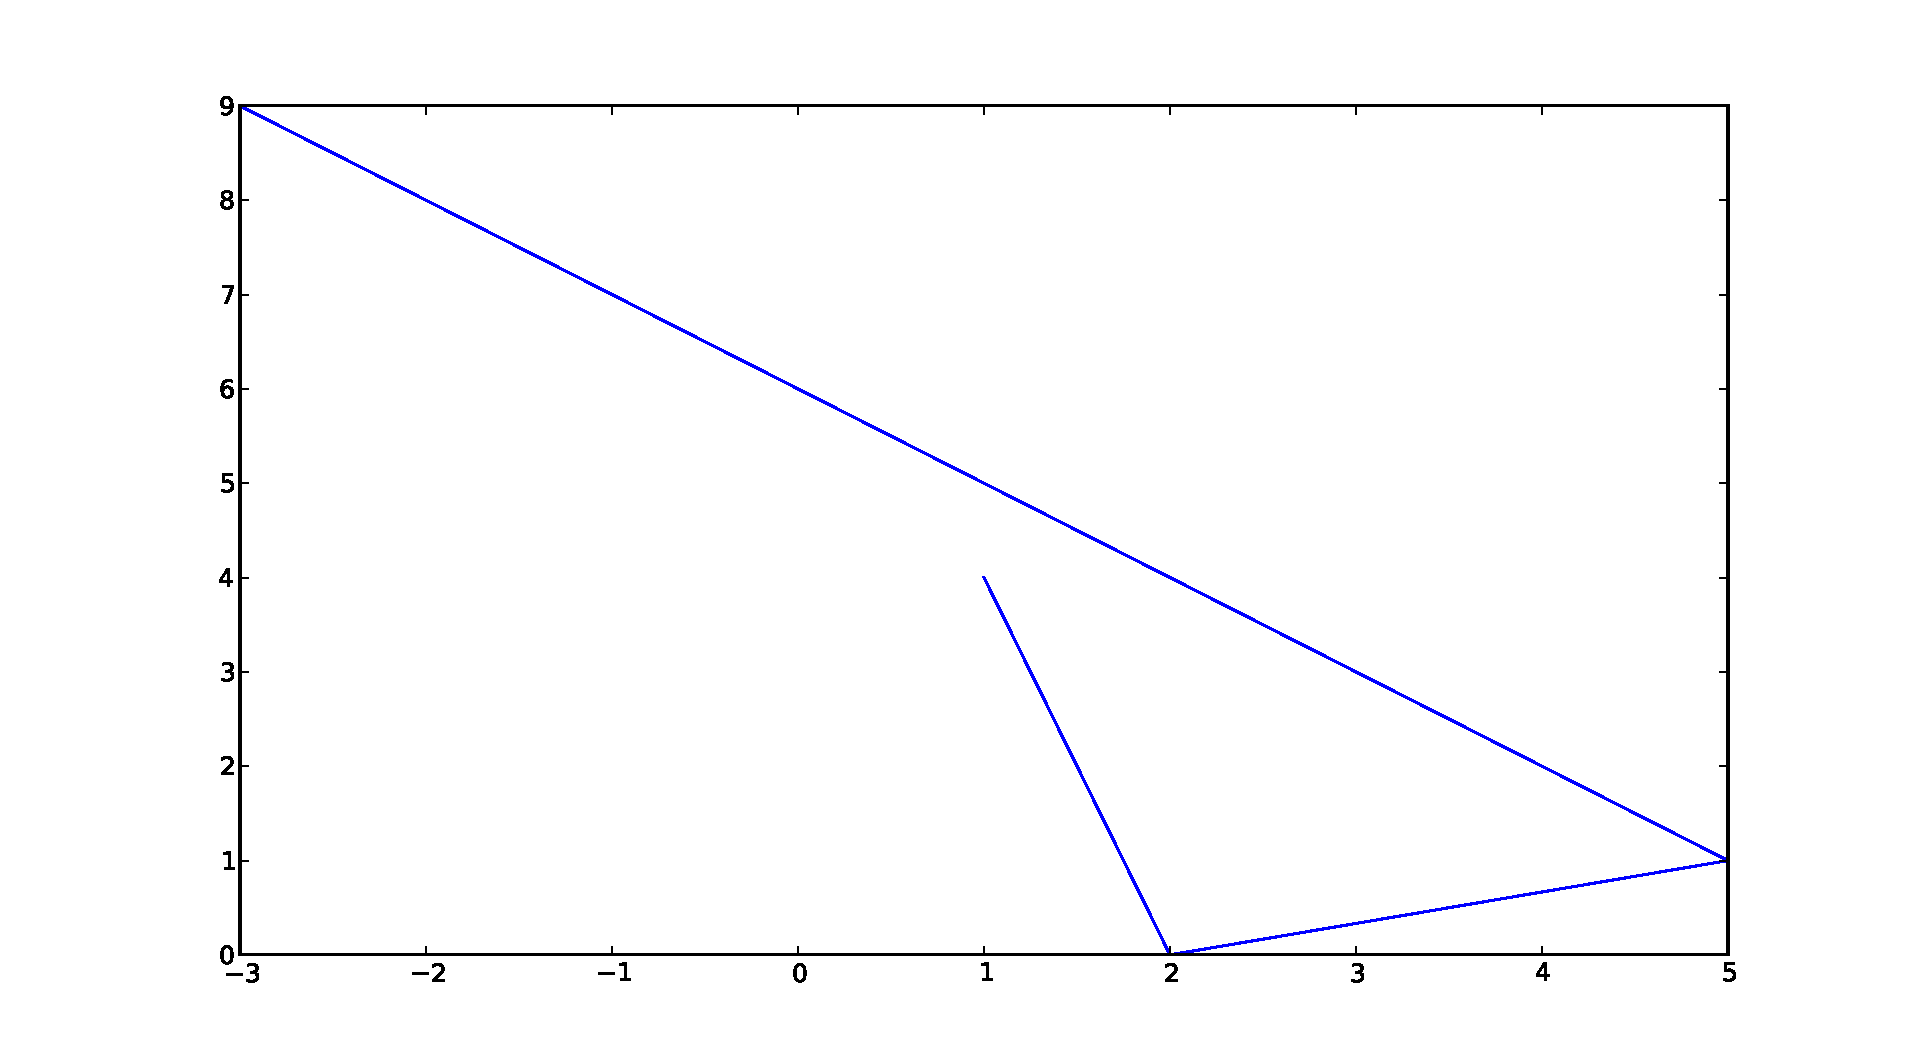
\includegraphics[scale=0.4]{first-plot}
  \caption{\label{fig:first-plot}Unser erster Plot mit Python.}
\end{figure}

Auf diese Weise kann man also \emph{Vektoren gegen Vektoren} plotten --
irgendwelche~$x$-Werte gegen irgendwelche~$y$-Werte. Wenn man
\emph{Funktionsgraphen} erstellen möchte, muss man selbst Hand anlegen:

\begin{minted}{python}
import numpy as np
import matplotlib.pyplot as pl

xs = np.linspace(0, 7, 300)
ys = np.sin(xs)

pl.plot(xs, ys)
pl.show()
\end{minted}

Dieser Code erzeugt Abbildung~\ref{fig:sine-graph}. Während wir im vorherigen
Beispiel manuell eine Liste von~$x$-Koordinaten eingaben, übernimmt das
jetzt die Methode~\mintinline{python}{np.linspace}. Sie erzeugt gleichmäßig
verteilte Stellen zwischen zwei Werten. Das kann man gut in der interaktiven
Python-Shell erkennen:
\begin{verbatim}
>>> np.linspace(3, 7, 10)
array([ 3.        ,  3.44444444,  3.88888889,  4.33333333,  4.77777778,
        5.22222222,  5.66666667,  6.11111111,  6.55555556,  7.        ])
\end{verbatim}
In Zeile~5 rufen wir die Sinusfunktion auf -- und zwar für jeden~$x$-Wert in
der Variablen~\mintinline{python}{xs} einmal. Die NumPy-Bibliothek, die wir
verwenden, nimmt uns dabei das Schreiben der eigentlich dafür benötigten
For-Schleife ab und erlaubt uns die bequeme Notation.
\begin{verbatim}
>>> np.sin(np.linspace(3,7,10))
array([ 0.14112001, -0.29824342, -0.67965796, -0.9290145 , -0.99786291,
       -0.8728259 , -0.57819824, -0.17122628,  0.26901506,  0.6569866 ])
\end{verbatim}

\begin{figure}
  \centering
  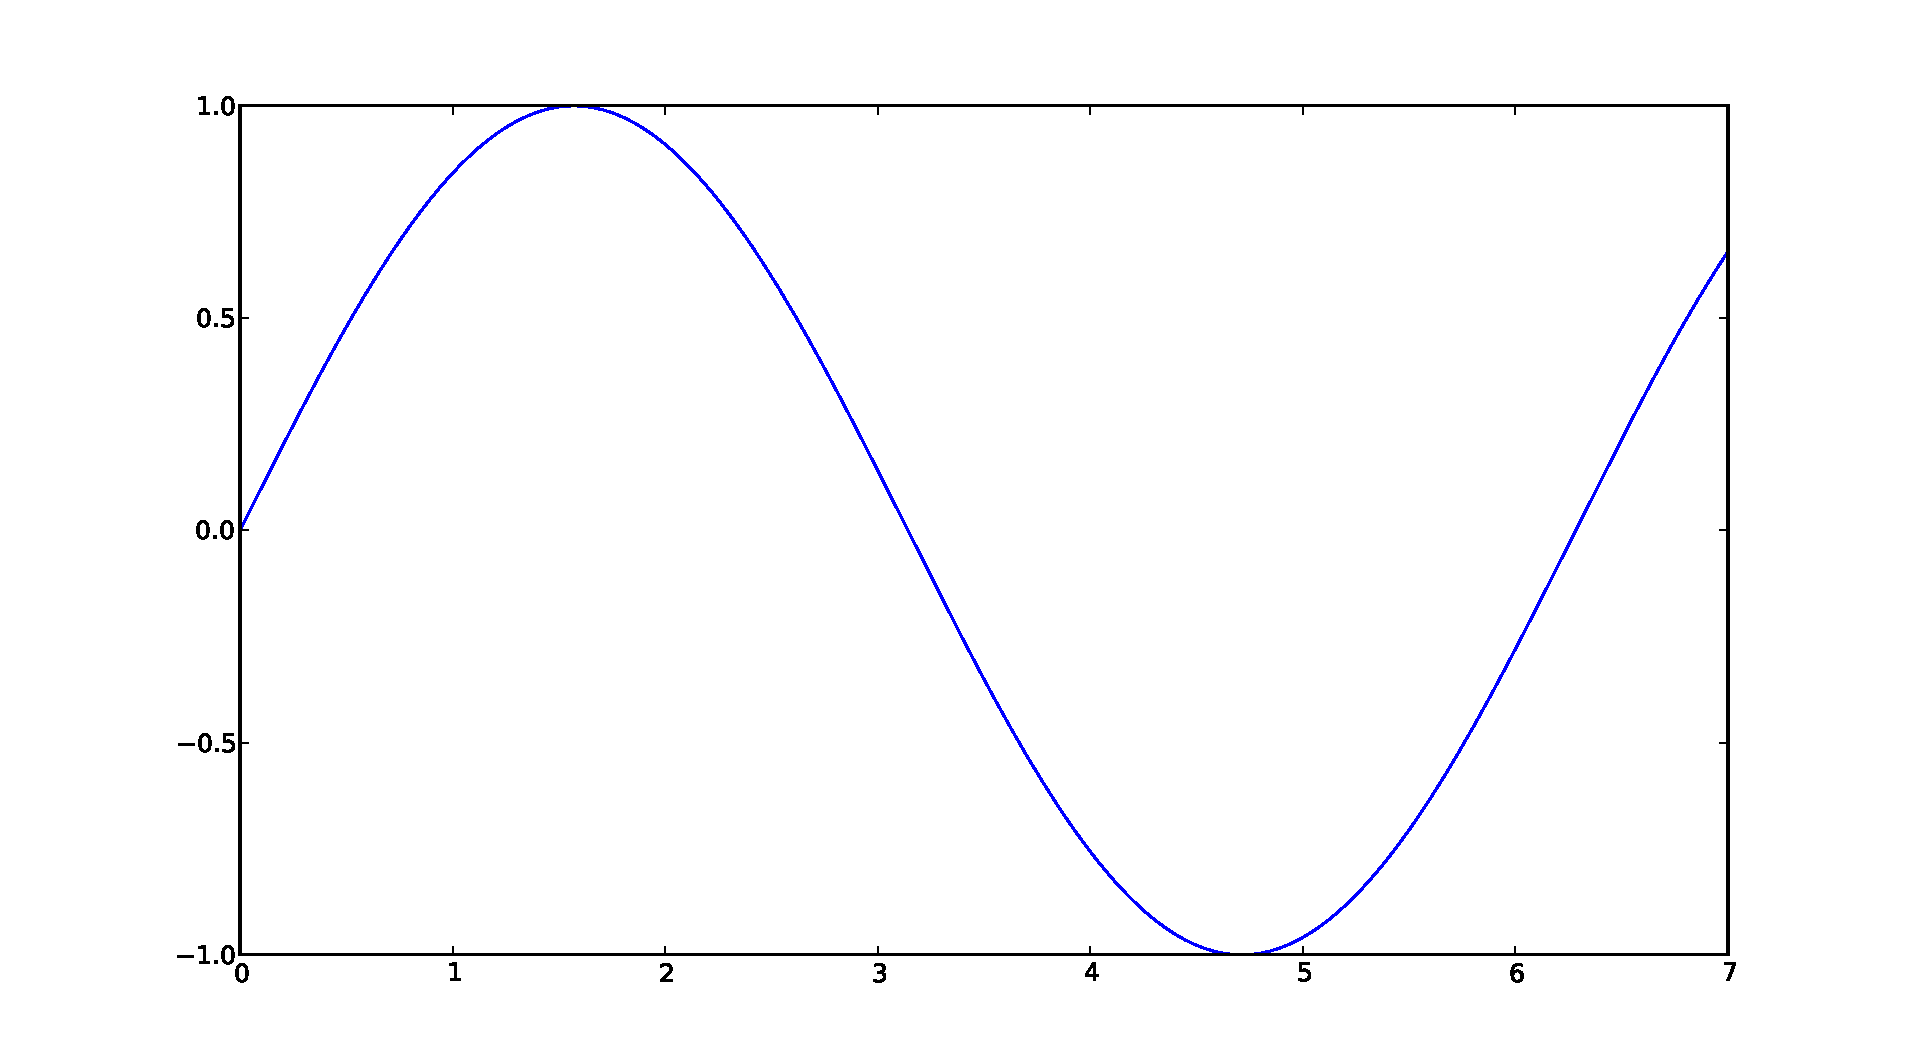
\includegraphics[scale=0.4]{sine-graph}
  \caption{\label{fig:sine-graph}Die Sinus-Funktion.}
\end{figure}



\section{Noch auszuarbeiten}

\begin{itemize}
\item Plotten. Dabei deutlich machen, dass man nicht Funktionen, sondern
Vektoren von $x$- und $y$-Werten gegeneinander plottet. Sowohl anonyme als auch
benannte Funktionen einführen. Als Beispiel vollständigen Programmcode liefern,
der eine Sinuskurve plottet. Auch auf dreidimensionale Plots eingehen.
\item Ableitungen numerisch berechnen.
\item Online-Python-Lösungen prüfen.
\item Deadline für diese Punkte: Ende Februar
\item Für später, auch in Abhängigkeit der Mathe-Blätter: Newton-Verfahren.
\end{itemize}

\end{document}
